\section{Systembeskrivelse}
Denne sektion vil beskrive hvordan systemet er sat op, samt hvilke chips og boards der er udleveret.
Til projektet er der anvendt det tildelte pan/tilt-system som har påmonteret et protection board, 2 hall sensorer, 2 h-broer og 2 motorer, der sidder på hhv. pan og tilt.\\
Til at styre denne opstilling er der udleveret èt stk Field Programmable Gate Array (FPGA) og èn Micro processor unit (MPU).
\\

\subsection{Fysiske begrænsninger}

Det udleverede pan- og tilt-system har fysiske begrænsninger i form af både range of motion, og de bælter der forbinder de to motorer med den fysiske ramme. Bælterne kan kamme over hvis de bliver tilført for stort kraftmoment, og pan-rammen har ikke mere end 180° graders frihed på den ene akse, grundet ledninger der nødvendigvis skal være forbundet til tilt-rammen.

\subsection{Micro Processor Unit}
Det udleverede Launchpad board som er et EK-TM4C123GXL board, er fra Texas Instruments. Den har en påmonteret MPU som er af modellen TM4C123GH6PM, denne er en Arm Cortex M4 chip \cite{TM4C123GH6PMDatasheet}.\\
Launchpad boardet får strøm gennem micro USB porten som sidder i øverste venstre hjørne som ses på figur \ref{fig:TivaLaunchPad}.\\
Micro USB porten bruges samtidig til at programmere boardet ved hjælp af et Integrated Development Environment (IDE). Til dette projekt blev Code Composer Studio \textsuperscript{\texttrademark} anvendt, som er Texas Instruments egen IDE.

\begin{figure}[!ht]
	\begin{center}
		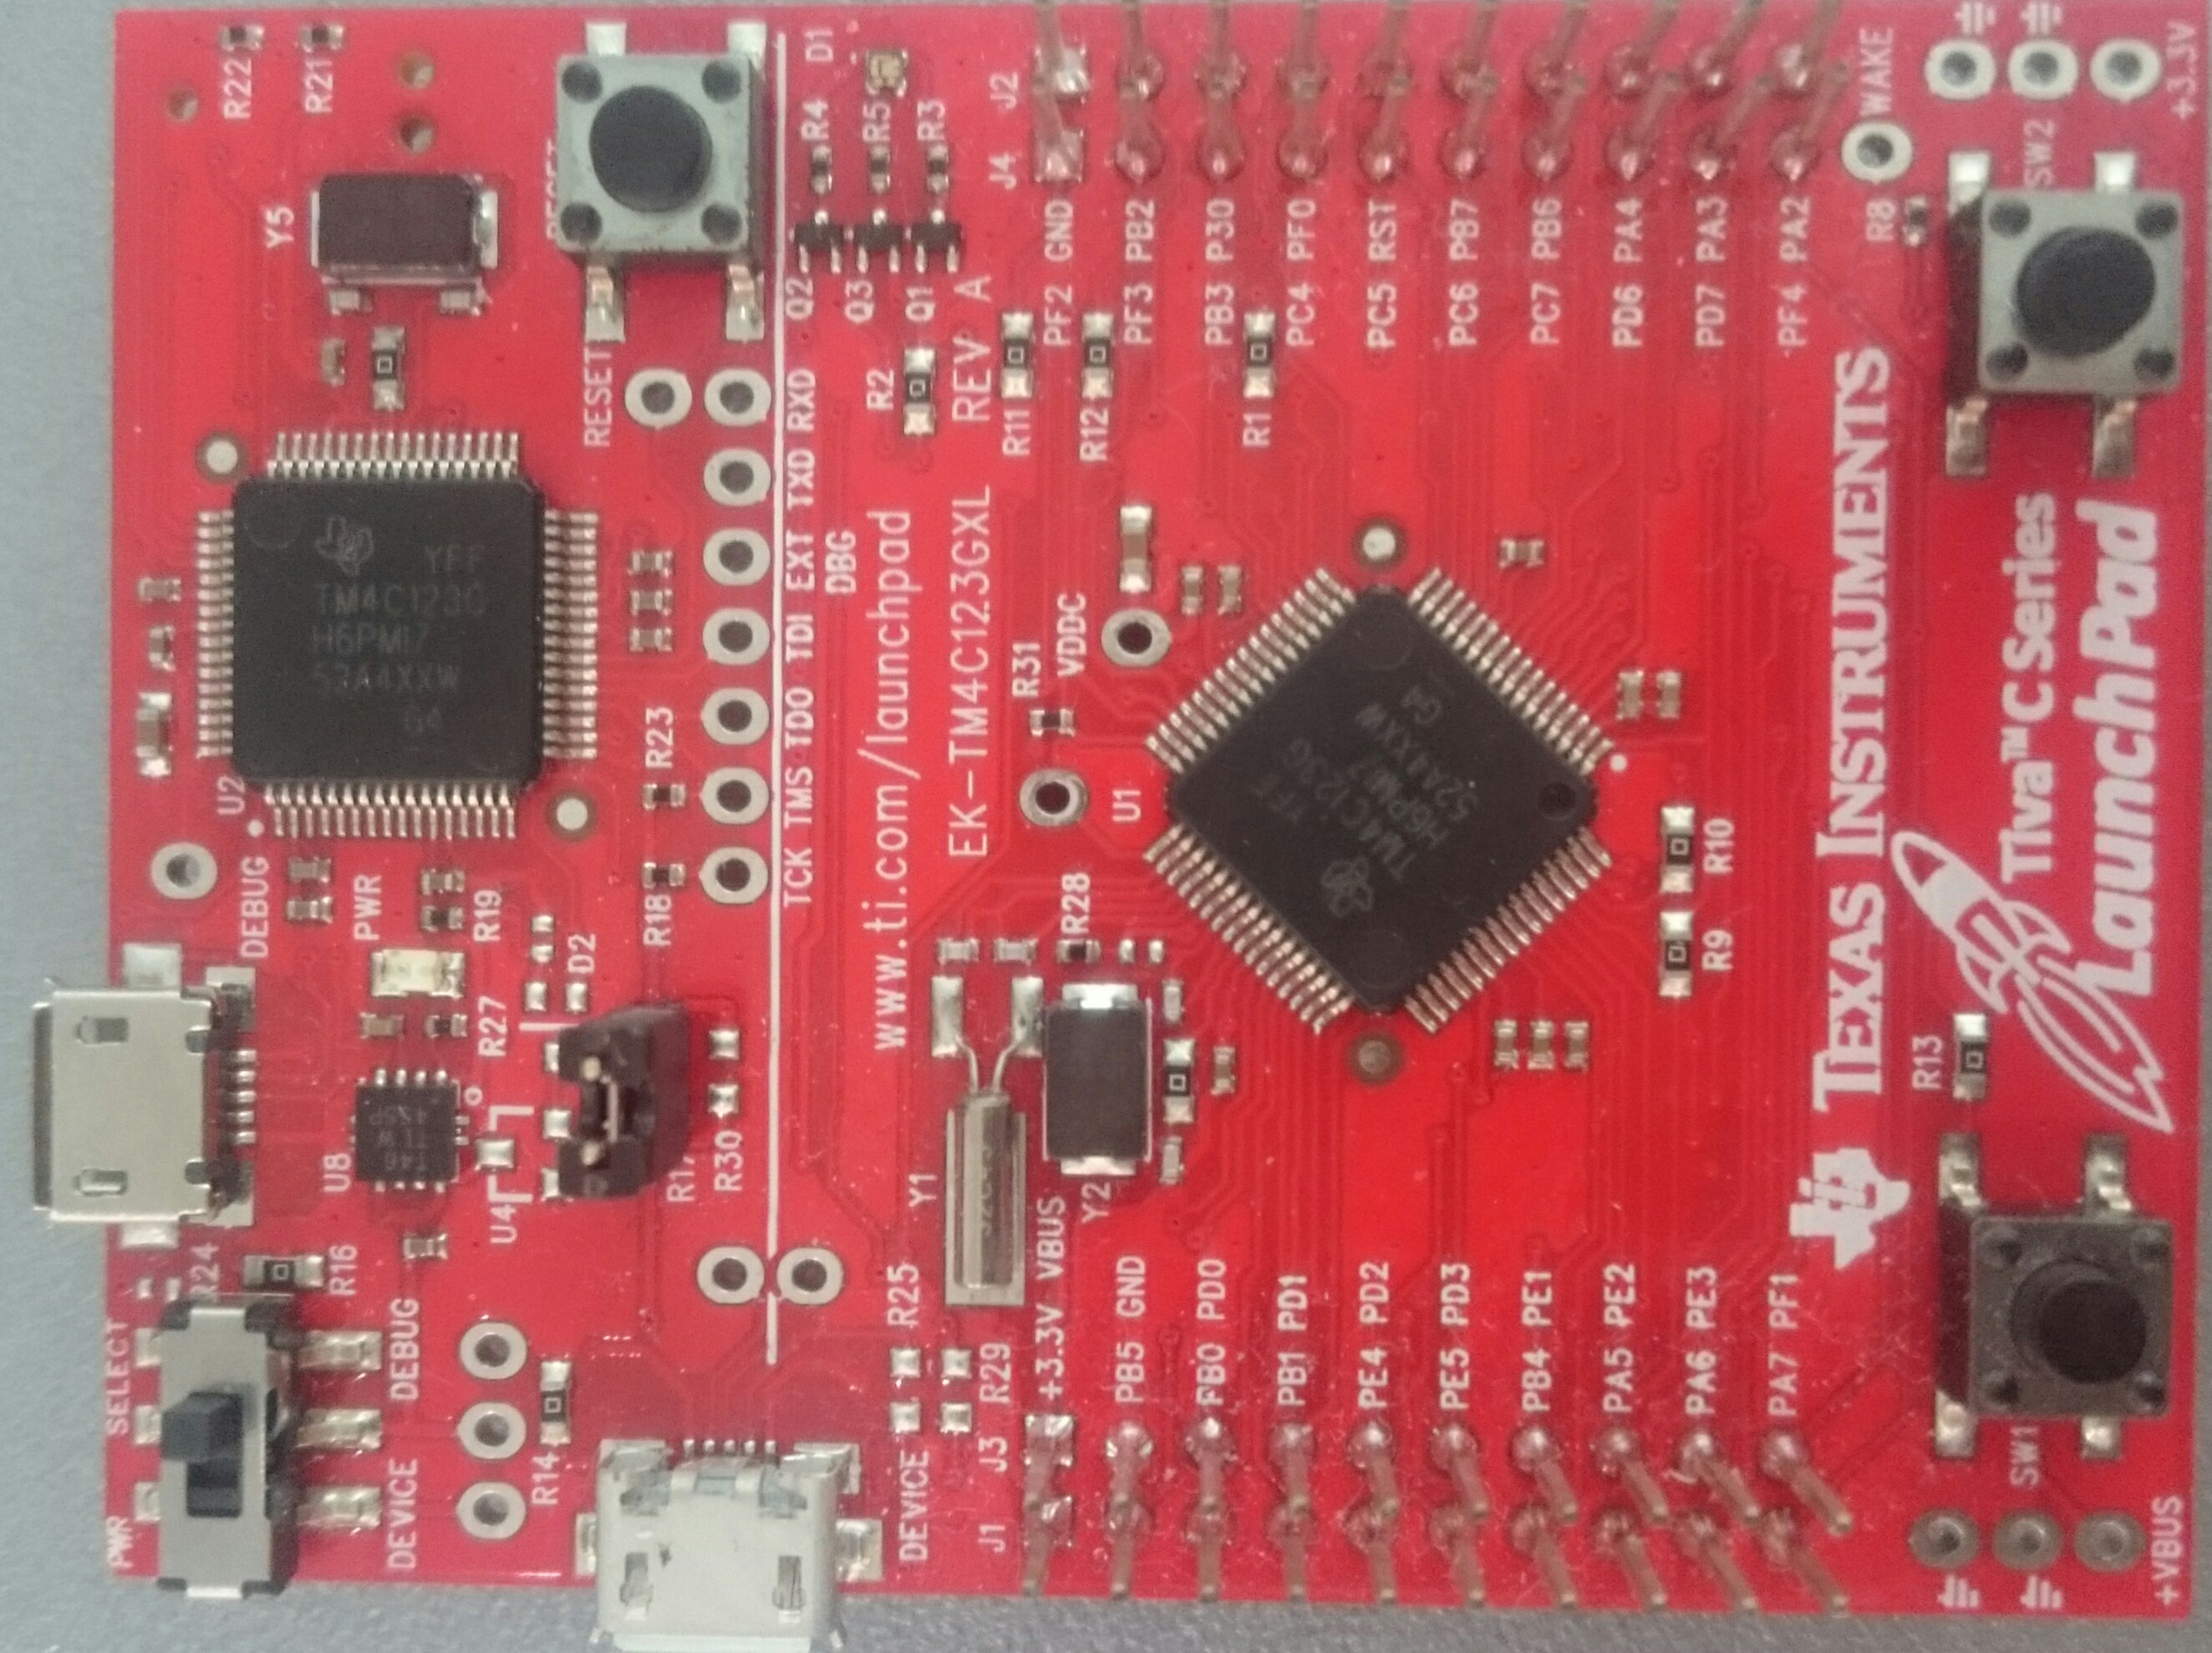
\includegraphics[scale=0.08, angle =270]{Billeder/TivaLaunchPad.JPG}
	\end{center}
\caption{Tiva\textsuperscript{\texttrademark} Launchpad boardet med den tilføjede TM4C123GH6PM arm cortex M4 Micro Processor Unit}
\label{fig:TivaLaunchPad}
\end{figure}

Launchpad boardet kan tilføjes til et embedded programmerings-board som blev udleveret i starten af semesteret som inkluderer et keypad, et LCD og en drehimpulsgeber, samt en SPI-udgang som anvendes til projektet, se figur \ref{fig:EMP_BOARD} og se vedlagt USB disk for at finde datablad, for mere information.

\begin{figure}[!ht]
	\begin{center}
		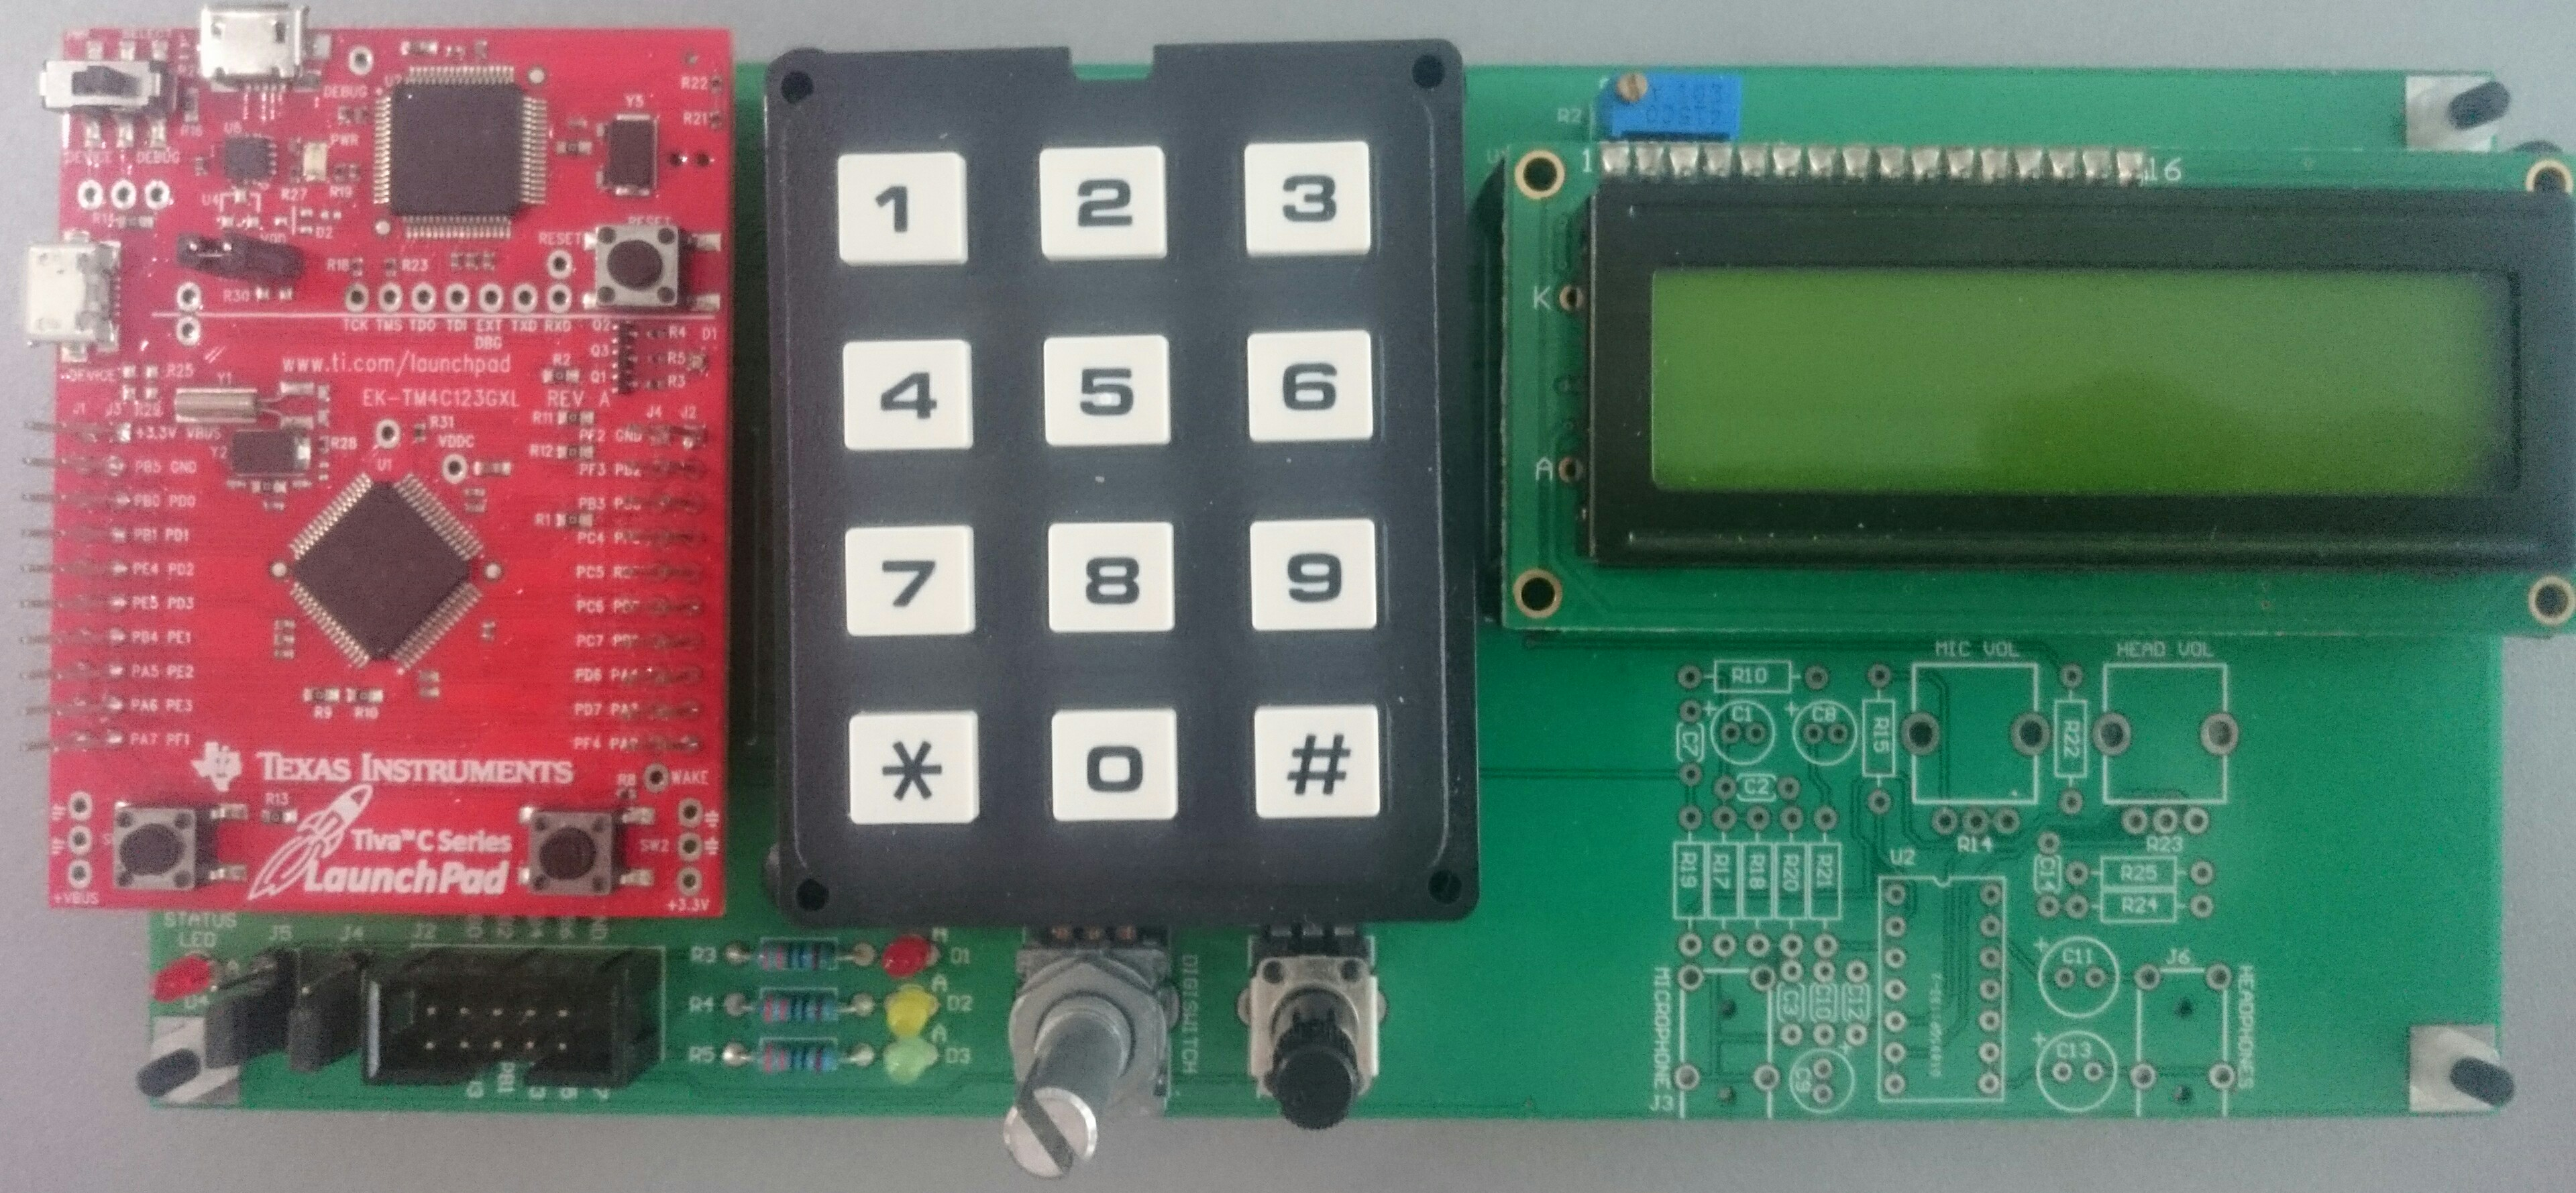
\includegraphics[scale=0.08, angle =0]{Billeder/EMP_BOARD.JPG}
	\end{center}
\caption{EMP Board med det tilføjede Launch pad board}
\label{fig:EMP_BOARD}
\end{figure}

\subsection{Field Programmable Gate Array}

Det udleverede board er en Nexys 2 af mærket Digilent, chippen som sidder på boardet er en Spartan-3E FPGA.

Nexys 2 boardet har fire 7-segment displays, med 8 switches og 4 knapper. Samtidig er der 3 porte som bliver brugt til projektet: JA,JC og JD.
Dette board får strøm og bliver programmeret igennem mini USB porten som sidder nede i venstre hjørne på figur \ref{fig:Nexys2Board}.
Mere information kan ses i databladet \cite{Nexys2Datasheet} på vedlagt USB nøgle.

\begin{figure}[!ht]
	\begin{center}
		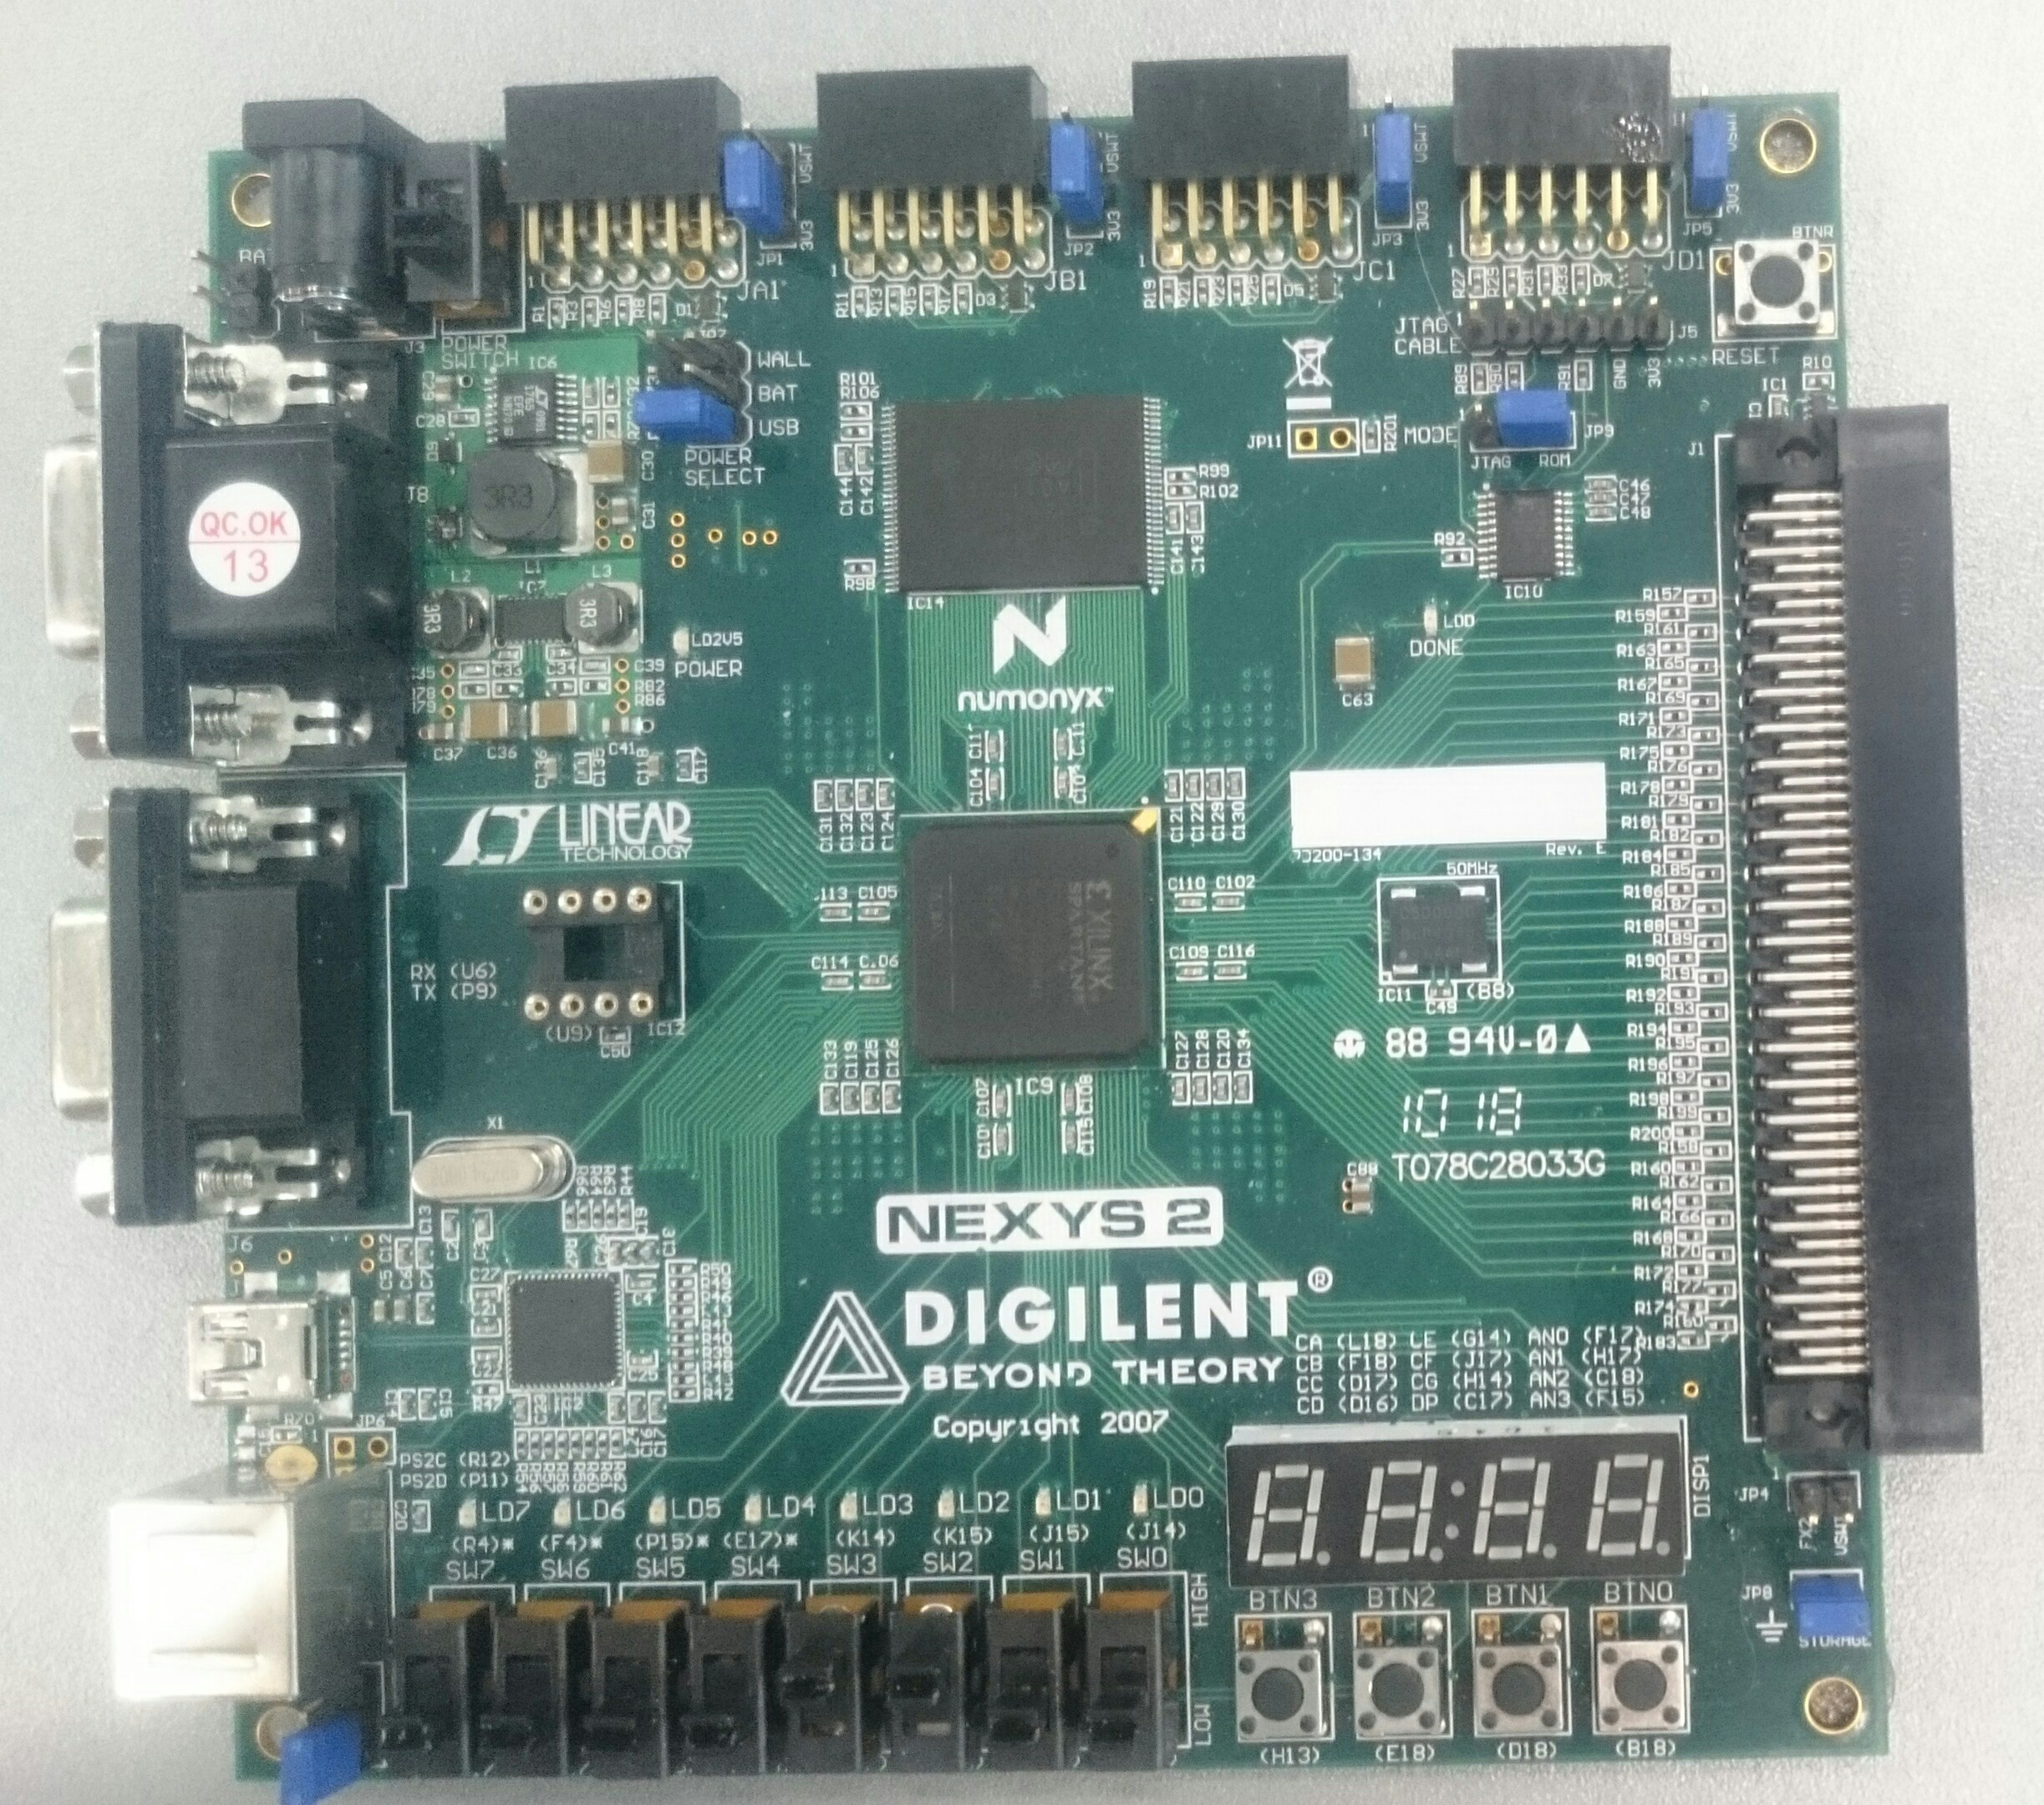
\includegraphics[scale=0.08, angle =0]{Billeder/Nexys2Board.JPG}
	\end{center}
\caption{Nexys 2 board med Spartan-3E FPGA'en}
\label{fig:Nexys2Board}
\end{figure}

\subsection{Intern kommunikations protokol}
Kommunikationen mellem MPU og FPGA skal foregå via Serial Peripheral Interface (SPI), som er en dataforbindelse som benytter fuld dupleks, altså hvor data kan sendes og modtages samtidig.
SPI foregår ved at der er en SPI master, og en eller flere slaver, kommunikationen sker derefter ved at masteren bestemmer hvilken slave som får lov til at sende sin data, for at der ikke opstår data kollision.

SPI gør brug af fire signaler til at kommunikerer med: MISO, MOSI, Clk og Slave Select.\\ 
MISO er data ud fra masteren. MOSI er data ind til masteren. Clk er den clock som bestemmer, hvornår data på MISO og MOSI er gyldig og kan clockes ind/ud. Og slave select er et signal der eksisterer per slave og som bruges til at vælge den slave der ønskes kommunikation med.


\subsection{Opsætning}
Pan- og tilt-motorerne er tilsluttet et protection board.\\
Protection boardet er tilsluttet de 2 H-broer samt FPGA'ens JC port.
De 2 H-broer er tilsluttet port JD på FPGA'en.
FPGA'ens JA port er tilsluttet MPU'ens port B som også er SPI (Se afsnit \ref{subsec:SPI}).